\documentclass[tikz]{standalone}

\usepackage{circuitikz}
\usepackage{physics}

\usetikzlibrary{calc,positioning}

\begin{document}
	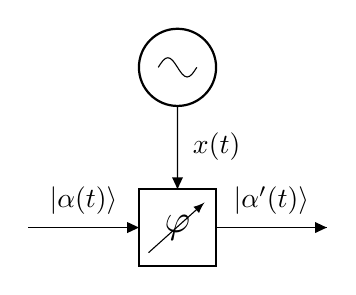
\begin{tikzpicture}[
		node distance=4em,
	]
		\coordinate (in) at (0,0);
		\node (phs) [vphaseshiftershape, right=of in] {};
		\node (osc) [vcoshape, above=3em of phs] {};
		\coordinate [right=of phs] (out);
		
		\draw (osc.south) to[short, l=$x(t)$] (phs.north) node[inputarrow, rotate=-90]{};
		\draw (in) to[short, l=$\ket{\alpha(t)}$] (phs.west) node[inputarrow]{};
		\draw (phs.east) to[short, l=$\ket{\alpha^\prime(t)}$] (out) node[inputarrow]{};
	\end{tikzpicture}
\end{document}
